\newcommand{\KAONS}{$K^{0}_{S}$}
\newcommand{\ANTILAMBDAS}{$\bar{\Lambda}$}
\newcommand{\XIMINUSS}{$\Xi^{-}$}
\newcommand{\XIPLUSS}{$\Xi^{+}$}
\newcommand{\mTS}{$m_{T}$}

\chapter{奇异粒子(\KAONS, $\Lambda$$+$\ANTILAMBDAS, \XIMINUSS+\XIPLUSS)的重构}
\section{介绍}
In these collisions, atomic nuclei (heavy-ions) moving at nearly the speed of light collide and deposit a large amount energy in a small region of space where the temperature and density is comparable with that existed in the early universe approximately on microsecond after the Big Bang.
These are six different types, or flavors, of quarks: $u$(up), $d$(down), $s$(strange), $c$(charm), $t$(top), $b$(bottom).
Nucleons only carry the lightest quarks $u$ and $d$.
The hadrons carrying strange quarks are strange hadrons.
Quarks have another important degree of freedom, known as color, just as electic charge to electrons.
A color is assigned to each quark,
for example, $R$(red), $G$(green) and $B$(blue).
All hadrons are colorless objects.
The forces between colored quarks are called strong interactions which is well described by Quantum ChromoDynamics(QCD).

\section{Nucleus-Nucleus Collisions Dynamics}
A high energy head-on nucleus-nucleus collision can be viewed in the laboratory frame as two thin disks approaching each other at nearly the speed of light because of the Lorentz contraction effect in the moving direction.
While a precise theoretical descrition of the collision dynamics is diffcult to find,
it is generally believed the ultra-relativistic heavy-ion collision has four stages of the evolution as shown in Fig. 1.4: pre-equilibrium parton cascade, an equilibrated QGP, hadronization and freeze-out of hadrons.
After the collision of two nuclei(Au $+$ Au at RHIC) at $(z, t) = (0, 0)$,
the energy density may be sufficiently high for the fromation of deconfined quarks and gluons,
a cascade of colliding partons.
This partonic state initically may not be in thermal equilibrium,
but the interaction between partons eventually bring the system into a local equilibrium at the proper time $\tau_{0}$ when the QGP is formed.
Then the QGP expands and its temperature drops down with increasing time.
The hadronization process takes places at a time in the order of \~ 10$\tau_{0}$.
This stage involves the formation of hadrons and hadrons continue to interact with each other.
As the system expanding further,
the interactions between the hadrons stop and the hadrons stream out of the collision region and the temperature falls below the freeze-out point.

Experimentally, since the direct probe of the QGP and hadronization process is not possible,
the measurement of the particles in the final stage is the only way for us to study the formation and evolution of the QGP at the early stages.
The initial energy density $\varepsilon$ right after the collision can be determined according to the produced particles.
\begin{figure}[hbtp]
  \centering
  \includegraphics[width=\linewidth]{pictures/pass.pdf}
  \caption{核核碰撞的时空演化图.}
  \label{fig:spaceTime}
\end{figure}
\begin{equation}
  \label{eq:S1}
  \varepsilon = \frac{m_{T}}{\tau_{0}A}\frac{dN}{dy}|_{y=0}.
\end{equation}
where $m_{T} = \sqrt{m^{2}+p_{T}^{2}}$ is the transverse mass of the particles produced,
$m$ and $p_{T}$ are the mass and the transverse momentum of the particles, respectively.
A is the overlapping area of two colliding nuclei and $\frac{dN}{dy}|_{y=0}$ is the number of hadrons pe unit rapidity.
The $\tau_{0}$, the proper time of thermalizing initial partons,
may depend on the colliding beam energy and is believed to be on the order of 1 $fm/c$.
For Au$+$Au collisions at RHIC,
most produced particles are pions.
The energy density $\varepsilon$ is about 4.6 $GeV/fm^{3}$ for Au$+$Au collision at $\sqrt{s_{NN}} = 130 GeV$ and $5.0 GeV/fm^{3}$ for $\sqrt{s_{NN}} = 200 GeV$ at RHIC.
These estimates of the energy density exceed the critical density for the QGP formation,
\~$1.0 GeV/fm^{3}$, calculated from lattice QCD.

\section{Collision Geometry}
Different from proton-proton collisions,
nuclear collisions can be reliably classified according to their centrality - a variable measuring the degree of overlapping between two colliding nuclei.
Centrality is closely related to the impact parameter $b$ that is defined as the transverse distance between the centers of the two colliding nuclei in a nucleus-nucleus collision as illustated in \ref{collision}.
\begin{figure}[hbtp]
  \centering
  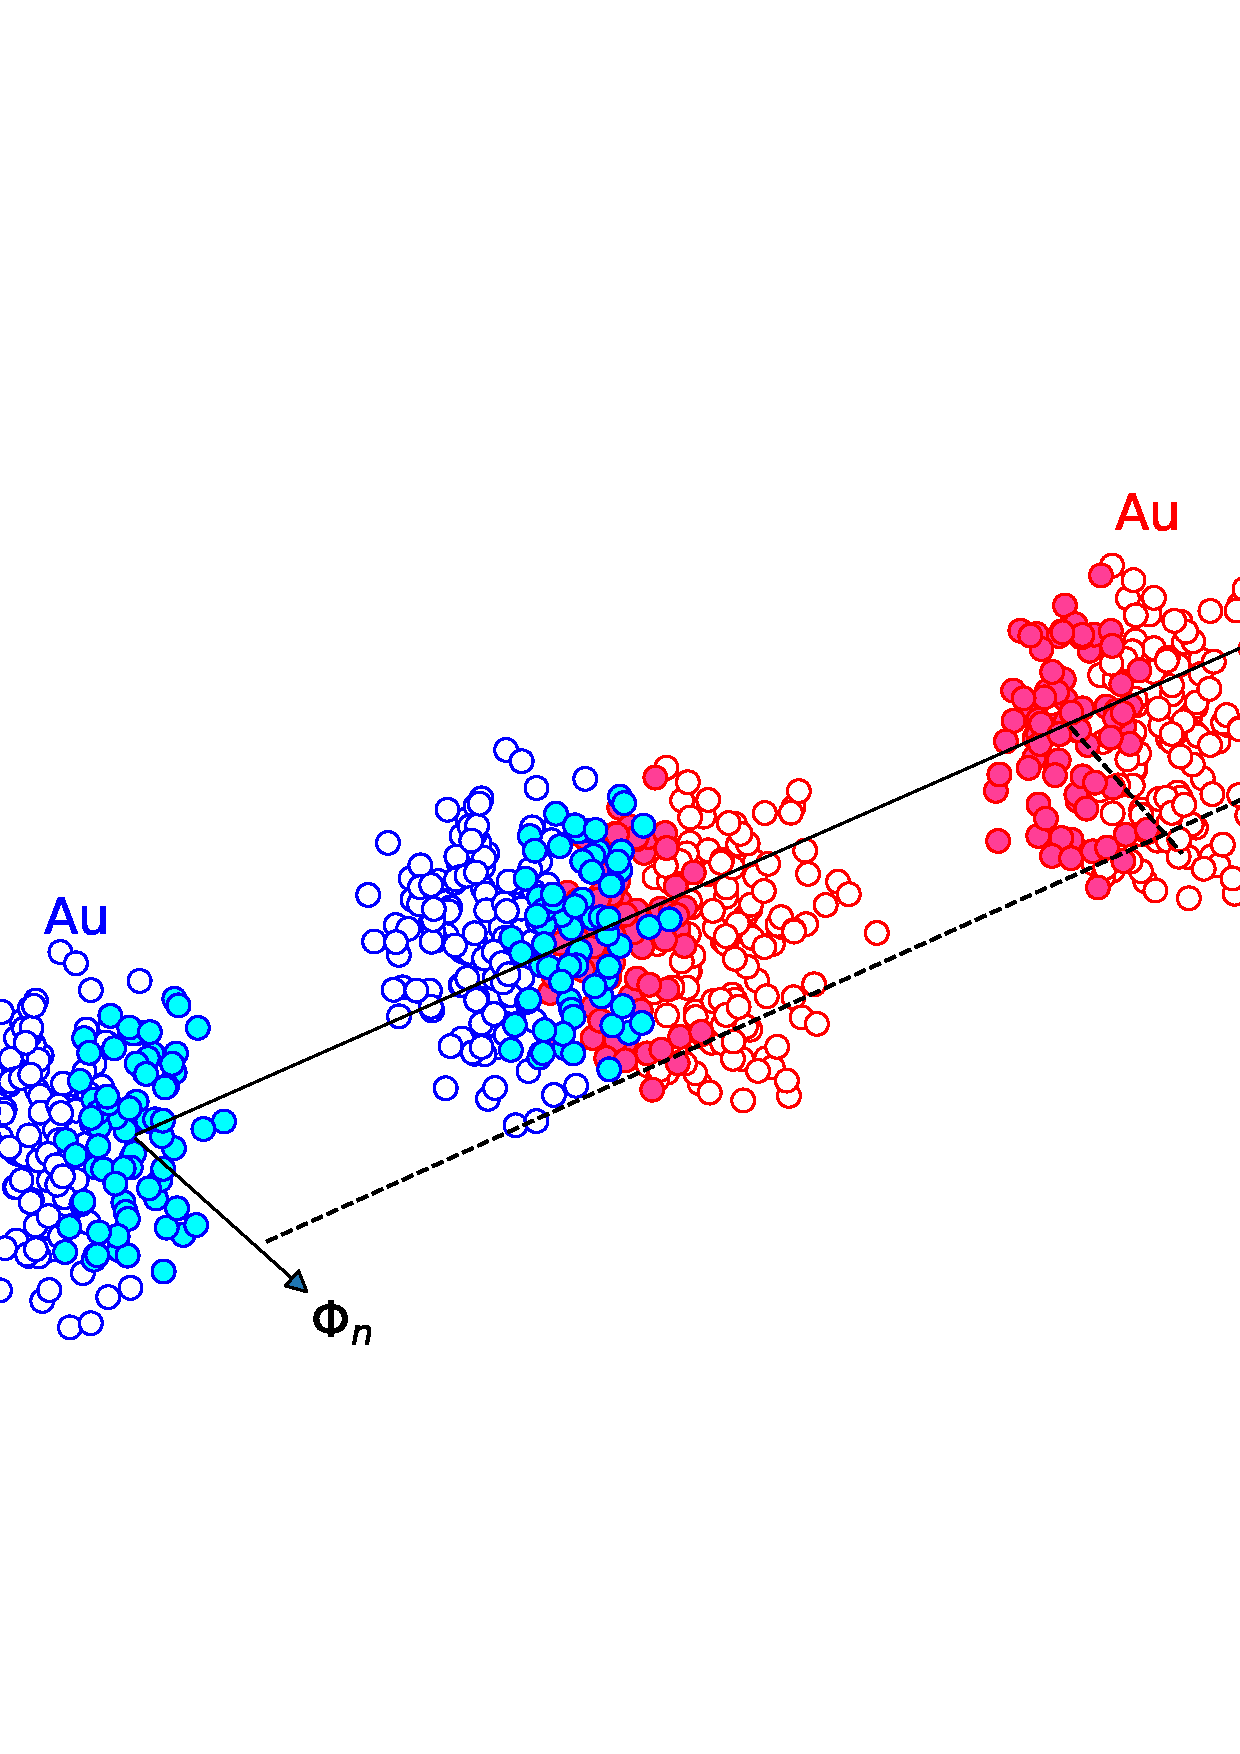
\includegraphics[width=\linewidth]{pictures/collision.pdf}
  \caption{Nuclear collision geometry and centrality for Au$+$Au collision.}
  \label{fig:collision}
\end{figure}
Althouth $b$ cannot be directly measured in experiments,
it has been widely used in theoretical models.
$N_{part}$ is another critical parameter in nuclear reactions and is a function of $b$.
Roughly speaking, a head-head collision with a small $b$ involves more colliding nucleons,
thus a large $N_{part}$.
For the most central collisions,
the impact parameter $b = 0$ and $N_{part} \approx A + A$.
The probability of this kind of collisions is very small, therefore corresponding to a top percentage (a few \%) of centrality.
Another similar collision parameter, $N_{binary}$, represents the number of equivalent nucleon-nucleon collisions in a nucleus-nucleus collision.
$N_{part}$ and $N_{binary}$ can be obtained from model calculations.
At STAR, the centrality is determined by measuring the charged particle multiplicity,
$N_{ch}$, for Au$+$Au and d$+$Au collisions.
Larger $N_{ch}$ corresponds to more central collisions.
For example, in Au$+$Au $200 GeV$ collisions the  centrality $0-5\%$ at STAR means the top 5\% events that have the averaged $N_{ch} > 686$ in middle rapidity region($|y| < 0.5$).

\section{Transverse Mass(Momentum) Spectra}
In heavy-ion collisions people are more interested in the invariant transverse mass(momentum) spectrum at a specific rapidity region,
\begin{equation}
  \label{eq:S2}
  \frac{d^{2}N}{2\pi{}p_{T}dp_{T}dy}
\end{equation}
At low $p_{T}$(< 2 GeV/c) in nucleus-nucleus or $p(d)$-nucleus collisions,
the spectrum can be well fitted by an exponential function in $m_{T}$
\begin{equation}
  \label{eq:S3}
  \frac{d^{2}N}{2\pi{}m_{T}dm_{T}dy} \propto e^{-\frac{m_{T}-m}{T}}.
\end{equation}
according to thermal models in which a large body of thermal hadronic or patonic matter is thought to act as a source of produced particles.
The fit parameter $T$, usually called temperature, is directly related to the freezeout temperature.
A large T means a earlier freezeout for a specific particle.
The heavy multi-strange hadrons, like the $\Omega$ and charmed hadrons, are good particles for probing the QGP since they have large $T$ and thus carry early early evolution information,
probably at the stage of the chemical freeze-out.
The hydrodynamic models have been successfully used to described the collective flow behavior at the low $p_{T}$ region.
The evolution of the flow is treated as an ideal fluid.
The flow velocity can be obtained by fitting the spectrum with Blast wave function.

然而,对于高$p_{T}$(> 2 GeV/c)区间,热模型核流体模型都无法较好的进行解释.
微扰QCD(pQCD)运用parton scattering, gluon shadowing and jet quenching等方法可以进行有效的描述.
这些方法导致一个较硬的$p_{T}$谱(更加的平缓),其谱的分布可以被指数函数进行拟合
\begin{equation}
  \label{eq:1}
  C(1+\frac{p_{T}}{p_{0}})^{-n}
\end{equation}
In the heavy-ion collisions, any approach trying to reproduce the experimental data successfully has to deal with the dominant dynamical mechanism for the {color{red} low $p_{T}$(soft) and high $p_{T}$(hard) region separately.}

\section{核的修正因子$R_{CP}$和$R_{AA}$}
It is believed that the QGP would be more likely to be created in central nucleus-nucleus collisions.
In peripheral collisions, where hte number of effect colliding nucleons is small,
the created matter is not sufficiently large to reach thermalization.
Nuclear effects can be investigated by measuring a nuclear modification factor,
the particle yield ratio from the central to peripheral collisions:
\begin{equation}
  \label{eq:2}
  R_{CP}(p_{T}) = \frac{[(dN/dp_{T})/N_{binary}]^{Central}}{[(dN/dp_{T})/N_{binary}]^{Peripheral}}
\end{equation}
其中,$N_{Binary}$是初始的核反应过程中,核核(nucleon-nucleon)碰撞的次数for each nuclear collision.
\begin{figure}[hbtp]
  \centering
  \includegraphics[width=\linewidth]{pictures/pass.pdf}
  \caption{$R_{CP}$的$p_{T}$依赖.}
  \label{fig:Rcp}
\end{figure}
类似于$R_{CP}$,另一个类似的核修正参数定义为核子碰撞的产额与质子碰撞的产额比.
\begin{equation}
  \label{eq:3}
  R_{AA}(p_{T}) = \frac{d^{2}N/dp_{T}d\eta}{T_{AA}d^{2}\sigma^{pp}/dp_{T}d\eta}
\end{equation}
其中$\eta$是赝快度,$T_{AA} = <N_{binary}>\sigma_{inel}^{NN}$.
$R_{AA}$取$pp$碰撞作为参考.

\section{Ehancement of Strange Hadrons}
A massive strangeness quark, $s$ 被认为对与QGP的信号是极其敏感的,因为其质量极其的靠近理论计算的相变临界温度值$T_{c}$,%
这就意味着奇异性强子的测量可以很好的提供退禁闭时的信息.
在退禁闭相时,奇异夸克可以通过($g+g -> s\bar{s}$)来产生,
通过该胶子反应道,奇异性核子产额的增多被认为是QGP存在的验证探针.

\section{探测器}
Four kinds of charged particles, $\pi^{+}(\pi^{-}), K^{+}(K^{-}), p(\bar{p}), e(\bar{e})$ can be identified via the measurement of ionization energy loss ($dE/dx$) of the particle travelling across the TPC.
Other neutral and charged particles, like the $K^{0}_{s}, \Lambda(\bar{\Lambda}), \Xi^{-}(\Xi^{+})$ and $\Omega^{-}(\Omega^{+})$可以通过弱衰变进行重构.
The vector meson $\phi$ can be measured up to $p_{T} = 6 GeV/c$ using event-mixing technique.
The EMC, designed to measure high energy $(\geq 2 GeV)$ electrons and photons,
is used to identify some particles decaying to electrons and photons,
such as $\pi^{0}, \eta$ and $J/\Psi$.

\section{分析方法}
In the STAR TPC, four particles(electictrons, pions, kaons and protons) in the low $p_{T}$ region can be identified through their energy loss rate($dE/dx$) along their track in the TPC,
while other particles are reconstructed from them through decay channels.
$K^{0}_{S}, \Lambda, \Xi^{-}$ and their anti-particles decay to pions and protons through their weak decay channels.
These involves a relatively long decaying time leading to a large decay length.
Therefore, the daughter particles (pions and protons) were created at some point in space away from the primary vertex.
This feature can be used to get rid of much background and makes these strange hadrons easy to reconstruct.
\subsection{minimum bias data}
To remove trigger biases, the minimum bias also require a vertex-z cut within 50 cm of the TPC center.
Moreover, primary vertices (collision points) were not successfully reconstructed in some events due to the low multiplicity (number of particles from one event) in the TPC so that these events are useless.
\subsection{Centrality definition}
Nuclear effects are different for the different collision centralities,
which are related to the impact parameter $b$ of the collision in geometry.
In experiments we define the centrality according to the number of charged particles measured in a given rapidity region.
These tracks must be from minimum bias events with primary vertex found.
The qualified tracks for the centrality definition are the charged primary tracks with the following requirements:
\begin{itemize}
\item{fit points $>=$ number.(拟合点大于某个值).}
\item{某个快度或者赝快度区间.}
\item{$p_{T}$小于某个区间.}
\item{a distance of closest approach {\color{red}(DCA)} to the primary vertex 小于某个距离.}
\end{itemize}
\begin{figure}[htpb]
  \centering
  \includegraphics[width=\linewidth]{pictures/pass.pdf}
  \caption{RefMult}
  \label{fig:RefMult}
\end{figure}
根据 reference multiplicity ($N_{ch}$) 来定义中心度.

\subsection{径迹的选择}
There are two sets of tracks available for the analysis in the STAR.
\begin{description}
\item[Primary tracks] {Primary tracks requiring a distance of closest approach (DCA) to the primary vertex less than 3 cm {\color{red} are usually used for identification of particles originating at or very close to the primary vertex.}}
\item[Global tracks] {Global tracks that include all the TPC tracks {\color{red}are mainly used to reconstruct particles that decay at some point in space away from the primary vertex.}}
\end{description}
对于$K^{0}_{s}, \Lambda, \Xi^{-}$ 以及它们的反粒子,因为较长的衰变距离,所以一般使用Global tracks来做重构的分析.
The number of hit points for each track ranges from 8 to 45.
We required at least 16 hit points for a track of good quality and discarded short tracks that might be split from a track with a large number of hit points.
To reduce the background for these reconstructed particles, the $n\sigma$ criterion cuts on their daughter tracks is used.
\begin{description}
\item[$n\sigma$ criterion] A parameter describing how far the measured $dE/dx$ deviates from the theoretical value of a known particle.
\end{description}

\subsection{V0重构}
V0粒子的衰变道和衰变分支比见\ref{tab:V0decay}.
The fact that V0 particles decay at some point away from the primary vertex allows us to build the signals by applying appropriate topology cuts.下图为V0衰变的x-y平面示例图
\begin{figure}[htbp]
  \centering
  \includegraphics[width=\linewidth]{pictures/pass.pdf}
  \caption{V0decay}
  \label{fig:V0decay}
\end{figure}
The trajectory of the charged daughter tracks, is a helix, that is, a circle in the x-y plane  plus a constant velocity in the Z direction.

To find V0s, we first need to calculate the distance of closest approach(DCA) between two daughter tracks (DCA $P^{+} + P^{-}$). Theoretically DCS $P^{+} + P^{-}$ should be zero if two daughter particles are decayed from the V0.
Practically a distance tolerance is, however, allowed due to the track position resolution.
We allow this DCA to be less than 1 cm.
The detailed math derivation for calculating DCA $P^{+} + P^{-}$ was published in \cite{PhysRevLett.89.132301}.

Similarly, a tolerance is applied to the DCA between the V0 and the primary vertex (DCA\_V0\_PV) even for a V0 coming from the primary vertex.
\begin{itemize}
\item All the $K^{0}_{s}$ particles are assumed to have been produced at the primary vertex,
so we set the limit for $K^{0}_{s}$ DCA\_V0\_PV as 1cm.
\item {However, some of $\Lambda$($\bar{\Lambda}$)} can be produced at the secondary vertex via the $\Xi$($\bar{\Xi}$) weak decay channel, which forces us to use a larger DCA\_V0\_PV cut.
\end{itemize}

The other two DCAs, DCA of $P^{+}$ to primary vertex (DCA\_P$+$\_PV) and DCA of $P^{-}$ to primary vertex (DCA\_P$-$\_PV),
can be used to reduce the background efficiently by cutting away a large portion of primary tracks which have small DCA\_P$+$\_PV or DCA\_P$-$\_PV.

V0粒子的动量方向由径迹$P+$和径迹$P-$在衰变顶点的动量之和决定.
衰变长度表示为衰变顶点和初级顶点之间的距离.
V0的不变质量($m$)由daughter径迹的质量和动量决定:
\begin{equation}
  \label{eq:4}
  m = \sqrt{(\sqrt{m_{+}^{2} + P_{+}^{2}} + \sqrt{m_{-}^{2}} + P_{-}^{2})^{2} - P^{2}},
\end{equation}
其中$m_{+}(m_{-})$是正负径迹粒子的质量,
$P_{+}$是正径迹的动量,
$P_{-}$是负径迹的动量,
$P$是V0粒子在衰变顶点的质量.

\subsection{不变质量谱和背景估计}
The $K^{0}_{s}$, $\Lambda$ and $\bar{\Lambda}$ particles are not identified on a particle-by-particle basis.
There is a large background from
\begin{itemize}
\item{random combinations of unidentified daughter particles;}
\item{uncorrelated identified daughter particles.}
\end{itemize}
However, the yield can be estimated by counting the candidates within a mass window around the center of the signal peak above a fitted background line.
\subsubsection{背景估计的旋转法}
决定背景的一种可能方法是将所有的positive径迹绕着初级顶点旋转180度.
这种方法destorys all the secondary vertices and only combinatorial background is reconstructed for the invariant mass distribution.
We use a combination of a Gaussian function and a second order polynomial function to fit the invariant mass distributions.

\section{Mass width and shift}
 We studied the mass width and shift from the invariant mass plots as a function of $p_{T}$.
主要研究动量分辨率的影响.

\section{$\Xi^{-}\bar{\Xi}^{+}$的重构}
\begin{table}[hbtp]
  \centering
  \begin{tabular}{ccc}\hline\hline
    Particles & Decay Channel & Branching ration \\\hline
    $\Xi^{-}$ & $\Lambda\pi^{-}$ & 99.89\% \\\hline
    $\bar{\Xi}^{+}$ & $\bar{\Lambda}\pi^{+}$ & 99.89\% \\\hline\hline
  \end{tabular}
  \caption{V0Xi}
  \label{tab:V0Xi}
\end{table}
$\Xi^{-}(\Xi^{+})$的衰变道如上表\ref{tab:V0Xi}所述.
其中$\Lambda$($\bar{\Lambda}$)的重构要采取前面叙述的方法.
衰变的重构图如下:
\begin{figure}[hbtp]
  \centering
  \includegraphics[width=\linewidth]{pictures/pass.pdf}
  \caption{VOXi}
  \label{fig:VOXi}
\end{figure}
%%% Local Variables:
%%% mode: latex
%%% TeX-master: "chapter02"
%%% End:
